\section{Variationen / Erweiterungen zu PID-Reglern}

\subsection{Modifizierter PID-Regler in Parallelform}

\begin{minipage}[t]{0.4\columnwidth}
    \begin{center}
        \textbf{\myul{Parallelform (normal)}}
    \end{center}
    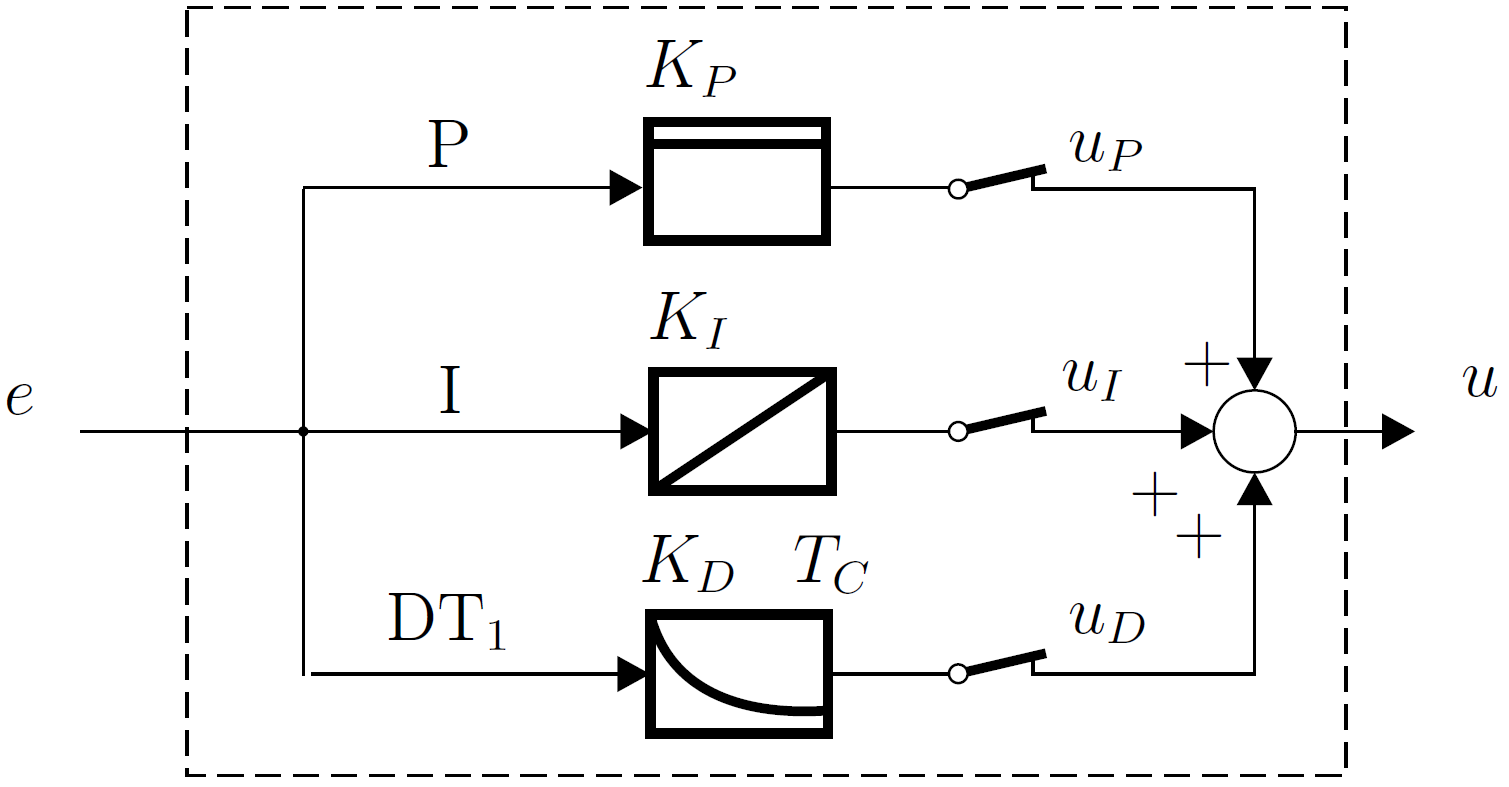
\includegraphics[width=\columnwidth]{images/pid_regler_aufbau.png}

    \textbf{Hinweis:} $P$-Anteil darf auch nach vorne gezogen werden (wie links) 
    \textrightarrow\ ändert Parameter von $I$- und $\text{DT}_1$-Gliedern
\end{minipage}
\hfill
\begin{minipage}[t]{0.55\columnwidth}
    \begin{center}
        \textbf{\myul{Modifizierte Form}}
    \end{center}
    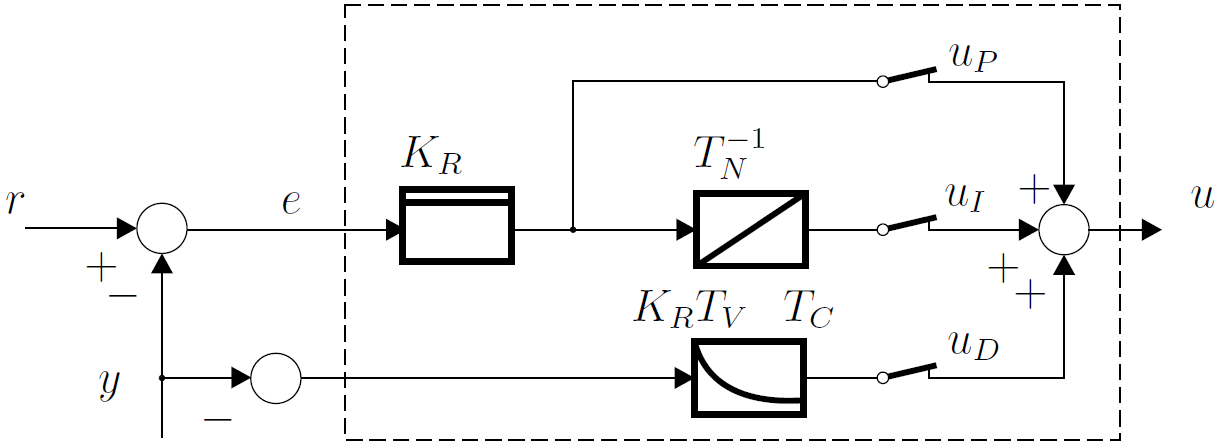
\includegraphics[width=\columnwidth]{images/modifizierter_pid_regler.png}

    Statt Fehler $e$ wird Ausgang $y$ auf $\text{DT}_1$-Glied geführt! \\
    \textrightarrow\ Ableitung des Ausgangs $y$ statt Ableitung des Fehlers $e$
\end{minipage}


\subsubsection{Eigenschaften / Auswirkungen der Modifikation}

\begin{minipage}[t]{0.48\columnwidth}
    \raggedright
    \begin{center}
        \textbf{\myul{Parallelform (normal)}}
    \end{center}

    \begin{outline}
        \1 Ändernde Referenz $r(t)$ (z.B. Sprung)
            \2 $\text{DT}_1$-Glied reagiert sehr aggressiv, da $e(t)$ gross \\
                \textrightarrow\ 'Überforderung' des Stellglieds
    \end{outline}

\end{minipage}
\hfill
\begin{minipage}[t]{0.48\columnwidth}
    \raggedright
    \begin{center}
        \textbf{\myul{Modifizierte Form}}
    \end{center}

    \begin{outline}
        \1 Ändernde Referenz $r(t)$ (z.B. Sprung)
            \2 $\text{DT}_1$-Glied reagiert nicht so aggressiv, da $y(t)$ 'träger' als $e(t)$ \\
                \textrightarrow\  Stellglied 'geschont'
        \1 'two degrees of freedom'
            \2 Reaktion auf Störung bzw. auf Änderung der Referenz separat einstellbar
    \end{outline}
\end{minipage}

\textbf{Achtung:} Der $\text{DT}_1$-Anteil kann nicht einfach weggelassen werden! 


\subsection{Glättung der Referenz}

\begin{minipage}[c]{0.3\columnwidth}
    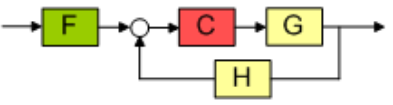
\includegraphics[width=\columnwidth]{images/filterung_stellgroesse.png}
    % \begin{center}
    \scalebox{0.4}{
    \begin{tikzpicture}
        [
            scale = 1,
            >=latex,
            orangebox/.style={rectangle, draw=black, fill=orange, thick, minimum width=1cm, minimum height=0.5cm},
            greenbox/.style={rectangle, draw=black, fill=green, thick, minimum width=1cm, minimum height=0.5cm},
            yellowbox/.style={rectangle, draw=black, fill=yellow, thick, minimum width=1cm, minimum height=0.5cm},
            whitecircle/.style={circle, draw=black, fill=white, thick, inner sep=0pt,minimum size=0.3cm},
        ]

        % nodes
        \node               (R)                                     {$r(t)$};
        \node[greenbox]     (F)       [right= of R]                 {F};
        \node[whitecircle]  (A)       [right= of F]                 {};
        \node[orangebox]    (C)       [right= of A]                 {C};   
        \node[yellowbox]    (G)       [right= of C]                 {G};
        \node[yellowbox]    (H)       [below left= of G]            {H};
        \node               (U)       [right= of G]                 {$u(t)$};

        % arrows
        \draw[->, thick]    (R)         to (F.west);
        \draw[->, thick]    (F.east)    to (A.west);
        \draw[->, thick]    (A.east)    to (C.west);
        \draw[->, thick]    (C.east)    to (G.west);
        \draw[->, thick]    (G.east) -> node {} coordinate(U-G) (U);
        \draw[->, thick]    (U-G)       to (H.east);
        \draw[->, thick]    (H.west)    to (A.south);        
    \end{tikzpicture}}
\end{center}
 #TODO fix drawing
\end{minipage}
\hfill
\begin{minipage}[c]{0.68\columnwidth}
    Die Stellgrösse $r(t)$ wird geglättet, um die Spitzenbelastung für das Stellglied zu mindern. Die wird erreicht, indem die 
    Stellgrösse mittels (\cgn{Filter F}) gefiltert wird. \textrightarrow\ Stellglied wird nicht überstrapaziert.
\end{minipage}



\subsection{Störgrössenaufschaltung}

\begin{minipage}[c]{0.55\columnwidth}
    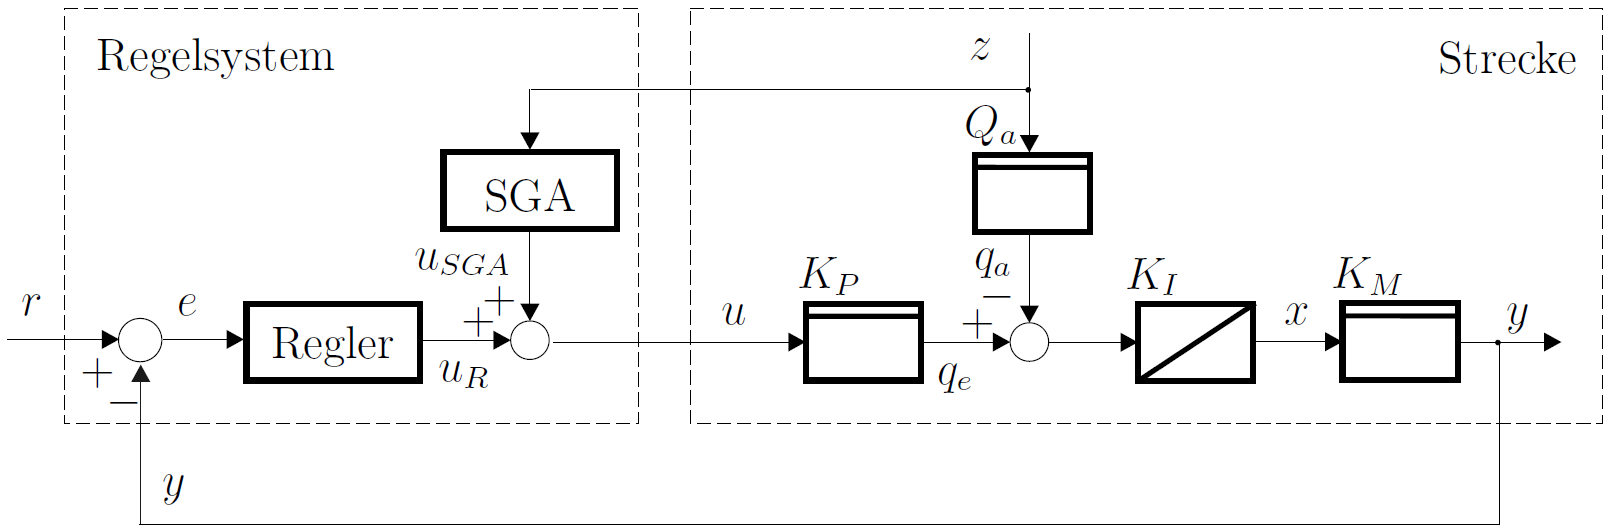
\includegraphics[width=\columnwidth]{images/stoergroessenaufschaltung.png}
    % \begin{center}
    \scalebox{0.63}{
    \begin{tikzpicture}
        [%
            scale = 1,
            >={Latex[length=1.5mm]},
            every node/.style={%
                font=\footnotesize, 
                rectangle, 
                draw, 
                minimum width=6mm, 
                minimum height=4mm
            },
            clearnode/.style={%
                rectangle, 
                draw=none, 
                fill=none, 
                minimum width=5mm, 
                minimum height=5mm, 
                inner sep=0pt
            },
            whitecircle/.style={%
                circle, 
                draw=black, 
                fill=white, 
                inner sep=0pt,
                minimum size=2mm
            },
        ]

        % nodes
        \node[clearnode]    (R)                         {$r(t)$};
        \node[fill=green]   (F)     [right=5mm of R]       {F};
        \node[whitecircle]  (A1)    [right=5mm of F]       {};
        \node[fill=orange]  (C1)    [right=5mm of A1]      {C1};   
        \node[whitecircle]  (A2)    [right=5mm of C1]      {};
        \node[fill=orange]  (C2)    [right=5mm of A2]      {C2};   
        \node[fill=yellow]  (G1)    [right=5mm of C2]      {G1};
        \node[fill=yellow]  (G2)    [right=5mm of G1]      {G2};
        \node[fill=yellow]  (H1)    [below=3mm of {$(A2.south west)!0.5!(G1.south east)$}] {H1};
        \node[fill=yellow]  (H2)    [below=3mm of H1]      {H2};
        \node[clearnode]    (U)     [right=5mm of G2]      {$u(t)$};

        % arrows
        \begin{scope}[every path/.style={->, thick}]
            \coordinate (G1G2) at ($(G1.east)!0.4!(G2.west)$);
            \coordinate (G2U) at ($(G2.east)!0.4!(U.west)$);
            
            \draw   (R)         to (F.west);
            \draw   (F.east)    to (A1.west);
            \draw   (A1.east)   to (C1.west);
            \draw   (C1.east)   to (A2.west);
            \draw   (A2.east)   to (C2.west);
            \draw   (C2.east)   to (G1.west);
            \draw   (G1.east)   to (G2.west);
            \draw   (G2.east)   to (U);
            \draw   (G1G2)      to (G1G2|-H1.east) to (H1.east); 
            \draw   (G2U)       to (G2U|-H2.east) to (H2.east); 
            \draw   (H2.west)   to (H2.west-|A1.south) to (A1.south);
            \draw   (H1.west)   to (H1.west-|A2.south) to (A2.south);
        \end{scope}
    \end{tikzpicture}}
\end{center} #TODO fix drawing
\end{minipage}
\hfill
\begin{minipage}[c]{0.43\columnwidth}
    Durch Messungen wird versucht, den Einfluss von Störungen $z(t)$ auf die Strecke gleich im Vornherein mittels 
    \cbl{SGA} zu kompensieren.
\end{minipage}

\begin{minipage}[t]{0.48\columnwidth}
    Am \cgn{grünen Knoten} gilt:
    $$ \dot{y} = K_M K_I [K_P u(t) - Q_a z(t)] $$

    Die Störung soll mittels \textbf{additiver Korrektur}
\end{minipage}
\hfill
\begin{minipage}[t]{0.48\columnwidth}
    
\end{minipage}


\subsection{Kaskadenregelung}

% \begin{center}
    \scalebox{0.63}{
    \begin{tikzpicture}
        [%
            scale = 1,
            >={Latex[length=1.5mm]},
            every node/.style={%
                font=\footnotesize, 
                rectangle, 
                draw, 
                minimum width=6mm, 
                minimum height=4mm
            },
            clearnode/.style={%
                rectangle, 
                draw=none, 
                fill=none, 
                minimum width=5mm, 
                minimum height=5mm, 
                inner sep=0pt
            },
            whitecircle/.style={%
                circle, 
                draw=black, 
                fill=white, 
                inner sep=0pt,
                minimum size=2mm
            },
        ]

        % nodes
        \node[clearnode]    (R)                         {$r(t)$};
        \node[fill=green]   (F)     [right=5mm of R]       {F};
        \node[whitecircle]  (A1)    [right=5mm of F]       {};
        \node[fill=orange]  (C1)    [right=5mm of A1]      {C1};   
        \node[whitecircle]  (A2)    [right=5mm of C1]      {};
        \node[fill=orange]  (C2)    [right=5mm of A2]      {C2};   
        \node[fill=yellow]  (G1)    [right=5mm of C2]      {G1};
        \node[fill=yellow]  (G2)    [right=5mm of G1]      {G2};
        \node[fill=yellow]  (H1)    [below=3mm of {$(A2.south west)!0.5!(G1.south east)$}] {H1};
        \node[fill=yellow]  (H2)    [below=3mm of H1]      {H2};
        \node[clearnode]    (U)     [right=5mm of G2]      {$u(t)$};

        % arrows
        \begin{scope}[every path/.style={->, thick}]
            \coordinate (G1G2) at ($(G1.east)!0.4!(G2.west)$);
            \coordinate (G2U) at ($(G2.east)!0.4!(U.west)$);
            
            \draw   (R)         to (F.west);
            \draw   (F.east)    to (A1.west);
            \draw   (A1.east)   to (C1.west);
            \draw   (C1.east)   to (A2.west);
            \draw   (A2.east)   to (C2.west);
            \draw   (C2.east)   to (G1.west);
            \draw   (G1.east)   to (G2.west);
            \draw   (G2.east)   to (U);
            \draw   (G1G2)      to (G1G2|-H1.east) to (H1.east); 
            \draw   (G2U)       to (G2U|-H2.east) to (H2.east); 
            \draw   (H2.west)   to (H2.west-|A1.south) to (A1.south);
            \draw   (H1.west)   to (H1.west-|A2.south) to (A2.south);
        \end{scope}
    \end{tikzpicture}}
\end{center}

% \subsection{Wind-Up}